%%%%%%%%%%%%%%%%%%%%%%%%%%%%%%%%%%%%%%%%%%%%%%%%%%%%%%%%%%%%%%%%%%%%%%%%%%%%%%%
% Chapter 3: Procedimiento experimental 
%%%%%%%%%%%%%%%%%%%%%%%%%%%%%%%%%%%%%%%%%%%%%%%%%%%%%%%%%%%%%%%%%%%%%%%%%%%%%%%

	A continuaci�n se proceder� a describir detalladamente el experimento llevado a cabo.
Se hablar� de en qu� consiste exactamente, en qu� se basa y como se ha planteado su
resoluci�n. Seguidamente, se enumerar� el material necesario para realizar la prueba.
Otro apartado estar� dedicado a mencionar los resultados que se han obtenido sin realizar
ninguna objeci�n sobre la implicaci�n de los mismos. Por �ltimo, se har� uso de los
conocimientos expuestos en el cap�tulo 2 para poder analizar los datos que hemos
obtenido y, as� mismo, lo que ello supone.

%++++++++++++++++++++++++++++++++++++++++++++++++++++++++++++++++++++++++++++++
\section{Descripci�n de los experimentos}
\label{3:sec:1}
	 Para la realizaci�n del experimento se ha utilizado b�sicamente un editor de texto
para escribir el c�digo fuente de Python y un int�rprete del mismo. El experimento consiste
en la realizaci�n de un programa en Python que sea capaz de calcular el valor de una integral
definida en un intervalo cerrado, que a su vez calcule su aproximaci�n por el m�todo de Simpson,
halle los errores relativo y absoluto entre los dos valores obtenidos y realice la representaci�n
gr�fica de la funci�n que se desea integrar y la par�bola generada por el m�todo utilizado
para su aproximaci�n. Como hemos mencionado anteriormente, se ha trabajado con una
funci�n dada ($f(x) = \frac{1}{1+e^{x}}$) definida en el intervalo $x \in [1, 6]$.

	Hay que considerar que la integral de f es $f'(x) = \ln{e^{x}} - \ln({e^{x}+1)}$ para poder
resolver la integral y hallar el valor real del �rea. Tambi�n debemos saber que la par�bola
que se ha de representar est� formada por los puntos f(a),f(b) y f($\frac{a+b}{2}$), por
lo que la ecuaci�n es $y = 0.0169x^2 - 0.17x + 0.422 $. 

%++++++++++++++++++++++++++++++++++++++++++++++++++++++++++++++++++++++++++++++
\section{Descripci�n del material}
\label{3:sec:2}
	En cuesti�n al material empleado para realizar el experimento se ha utilizado un
computador con un procesador Intel(R) Core(TM)2 Quad CPU Q6600 @ 2.40GHz 2.39 GHz y 
una memoria RAM de 3,00 GB. El sistema operativo que conten�a el computador era 
Windows 7 Home Premium de 32 bits. Para escribir los c�digos fuente de LaTeX se
usaron los programas Texmaker y Kate (versiones 3.2 y 3.8.5, respectivamente) y para 
el c�digo fuente de Python solamente se utiliz� Kate. Adem�s, para registrar los cambios
realizados en el trabajo y subirlos a GitHub se hizo uso de Git (1.7.9.5). Como 
compiladores se emple� el int�rprete de Python y el compilador de Tex.

%++++++++++++++++++++++++++++++++++++++++++++++++++++++++++++++++++++++++++++++
\section{Resultados obtenidos}
\label{3:sec:3}

bla, bla, etc. 


%------------------------------------------------------------------------------
\begin{figure}[!th]
\begin{center}
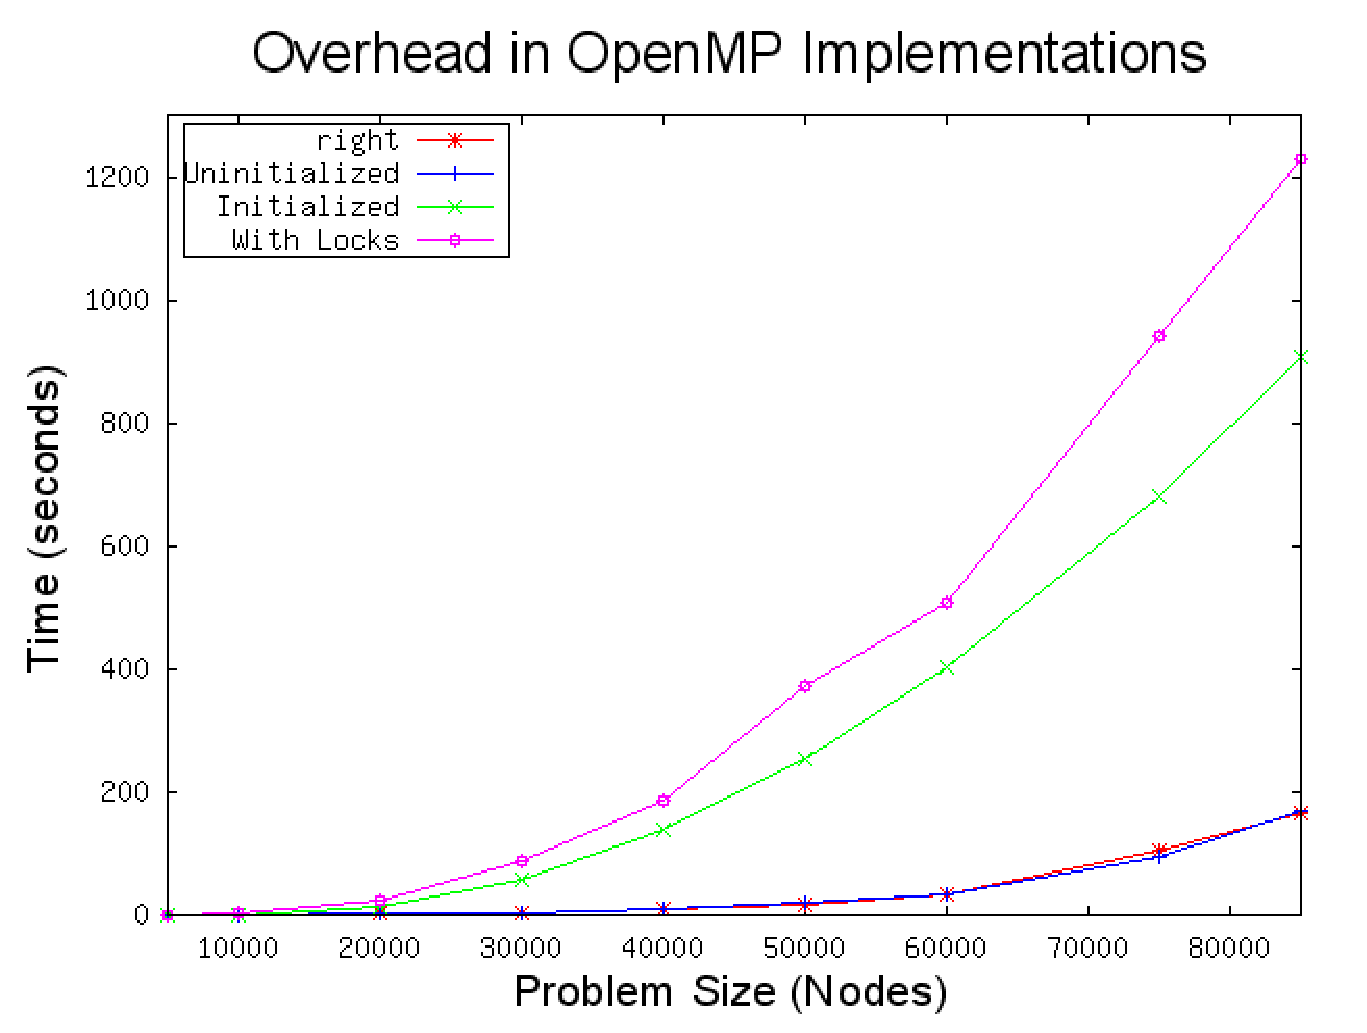
\includegraphics[width=0.75\textwidth]{mem/images/figura1.eps}
\caption{Ejemplo de figura}
\label{fig:1}
\end{center}
\end{figure}
%------------------------------------------------------------------------------


%------------------------------------------------------------------------------
%--------------------------------------------------------------------------
\begin{table}[!ht]
\begin{center}
\begin{tabular}{|c|c|} \hline 
\textbf{Tiempo  } & \textbf{Velocidad} \\ 
\textbf{($\pm$ 0.001 s)} & \textbf{($\pm$ 0.1 m/s)} \\ \hline \hline
1.234 &
67.8
\\
\hline

2.345 &
78.9
\\
\hline

3.456 &
89.1
\\
\hline

4.567 &
91.2
\\
\hline

\end{tabular}
\end{center}
\caption{Resultados experimentales de tiempo (s) y velocidad (m/s)}
\label{tab:1}
\end{table}


%------------------------------------------------------------------------------

%++++++++++++++++++++++++++++++++++++++++++++++++++++++++++++++++++++++++++++++
\section{An�lisis de los resultados}
\label{3:sec:4}

bla, bla, etc. 

